%------------------------------------------------------------------------------------------------------------------------
\chapter{電荷補正の最適化}
\label{sec:chap4}
%------------------------------------------------------------------------------------------------------------------------
Threshold、ToTのチューニングおよび電荷較正を行った後、それぞれのパラメータが適切な値を保持していることを確認しデータベースに必要なパラメータ情報の登録を行う。電荷較正では正しく結果を出力しない場合があるため、結果に適切な値を補完しデータベースにアップロードする。ATLASピクセル検出器に搭載されている非常に多くのFEチップに対して電荷較正が一括に行われるため、全てのFEチップについての結果に問題が無いかを確認する必要がある。
本研究では、電荷較正の際に発生するいくつかの問題に対し例外処理を行い、より適切な値に近い値を補完するアルゴリズムの開発を行った。
本章では、電荷較正で発生する問題と、その問題に対する処理方法について説明する。

%------------------------------------------------------------------------------------------------------------------------
\section{電荷較正における補正の概要}
\label{sec:hoseigaiyou}
%------------------------------------------------------------------------------------------------------------------------

電荷較正では、ピクセル検出器およびIBLに搭載された計28400個のFEチップを同時に操作するため、全てが正常に機能しないことがある。電荷較正における問題は主に以下の2つがあげられる。
%本節ではそれぞれについての問題の原因とこれまでの補完方法について説明する。

\begin{itemize}
  \item[1. ] 不適当な電荷を使った電荷較正
  \item[2. ] データの欠損
\end{itemize}

1つ目の問題に関して、ピクセルモジュールの電荷較正ではFEチップに搭載された回路を用いて試験電荷を生成し、ThresholdスキャンやToTスキャンを行う。電荷生成のための回路のいずれかの部分に故障等の問題があると、誤った試験電荷を生成してしまう。問題がある場合とない場合の試験電荷について、電荷較正\eref{eq:calibration}を用いてフィッティングした結果を\fref{fig:calibhikaku}に示す。\fref{fig:calibhikaku}において、左図は理想的なフィッティング結果を表しており、全ての点がフィット曲線上に乗っていることがわかる。この様に、ToTとセンサーが落とす電荷量は、おおよそ線形関係にあることがわかる。

\begin{figure}[tbp]
  \begin{minipage}[b]{0.5\linewidth}
    \centering
    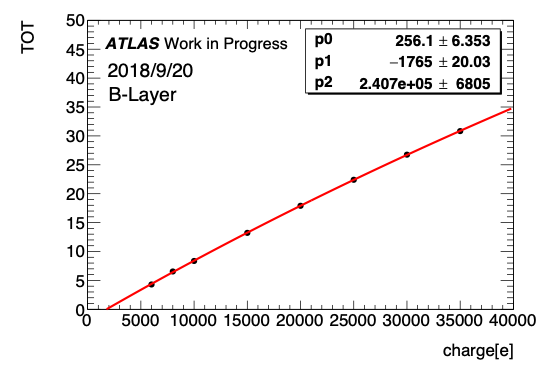
\includegraphics[keepaspectratio, scale=0.8]{goodcalib.png}
  \end{minipage}
  \begin{minipage}[b]{0.5\linewidth}
    \centering
    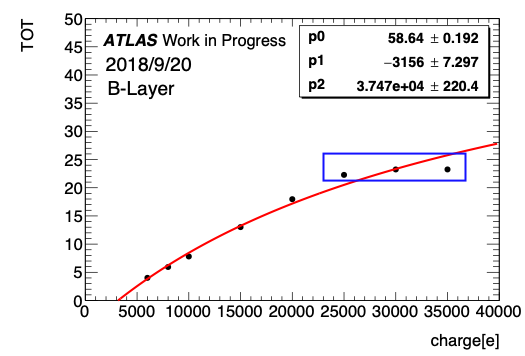
\includegraphics[keepaspectratio, scale=0.8]{badcalib.png}
  \end{minipage}
  \caption[電荷較正\eref{eq:calibration}を用いてフィッティングした結果]{電荷較正\eref{eq:calibration}を用いてフィッティングした結果。左図は理想的なフィッティング結果を表しており、右図は正しいToTが得られていない点を含むフィッティング結果である。}
  \label{fig:calibhikaku}
\end{figure}

一方で、右図は電荷生成の回路に問題のあるFEチップにおける電荷較正結果であり、電荷量の大きい3つの試験電荷についてToTの値がほとんど同じ値になっている。この原因は、試験電荷生成のための回路における電圧$V_\mathrm{cal}$の値が正しくキャパシタに渡されないことにある。$V_\mathrm{cal}$は\textbf{Plsr DAC}と呼ばれる$10\ \si{bit}$の値により決定される。$V_\mathrm{cal}$と$\mathrm{Plsr\ DAC}$の関係は\eref{eq:vcal}のように、1次式で与えられる。
\begin{equation}
  \label{eq:vcal}
  V_\mathrm{cal} = a + b\ (\mathrm{Plsr\ DAC})\ [\si{mV}]
\end{equation}
ここで、$a,\ b$は較正によって決定される定数であり、FEチップごとに個体差がある。あるFEチップに対する$V_\mathrm{cal}$とPlsr DACの関係の測定結果を\fref{fig:vcalplot}に示す。この図において、$\mathrm{Plsr\ DAC}\approx 750$までは$V_\mathrm{cal}$とPlsr DACの値が線形となっているが、それ以降のPlsr DAC値においては$V_\mathrm{cal}$が飽和していることがわかる。この$V_\mathrm{cal}$の飽和は、試験電荷生成回路におけるキャパシタ$C_\mathrm{low}$および$C_\mathrm{high}$の内、$C_\mathrm{low}$のみを用いて試験電荷を生成した場合に発生しやすいことがわかっている \cite{houwa}。\fref{fig:analog}に示したように、$C_\mathrm{high}$の前に配置されているスイッチを用いる事により使用するキャパシタの選択を行うことができる。電荷較正の際には、$C_\mathrm{low}$のみを用いるためこのスイッチは開放されているが、$V_\mathrm{cal}$の値が大きいときにはグランドへのリーク電流が大きくなってしまう。そのため、ある値以上の電荷を持つ試験電荷を正確に取得することができず、正しい電荷較正結果が得られない。$V_\mathrm{cal}$の飽和が起きていると予想される\fref{fig:calibhikaku}の右図の場合は、電荷較正に使用された試験電荷の内、正しいToTが得られていない2点を取り除き、再較正を行う必要がある。
\begin{figure}[tbp]
  \centering
  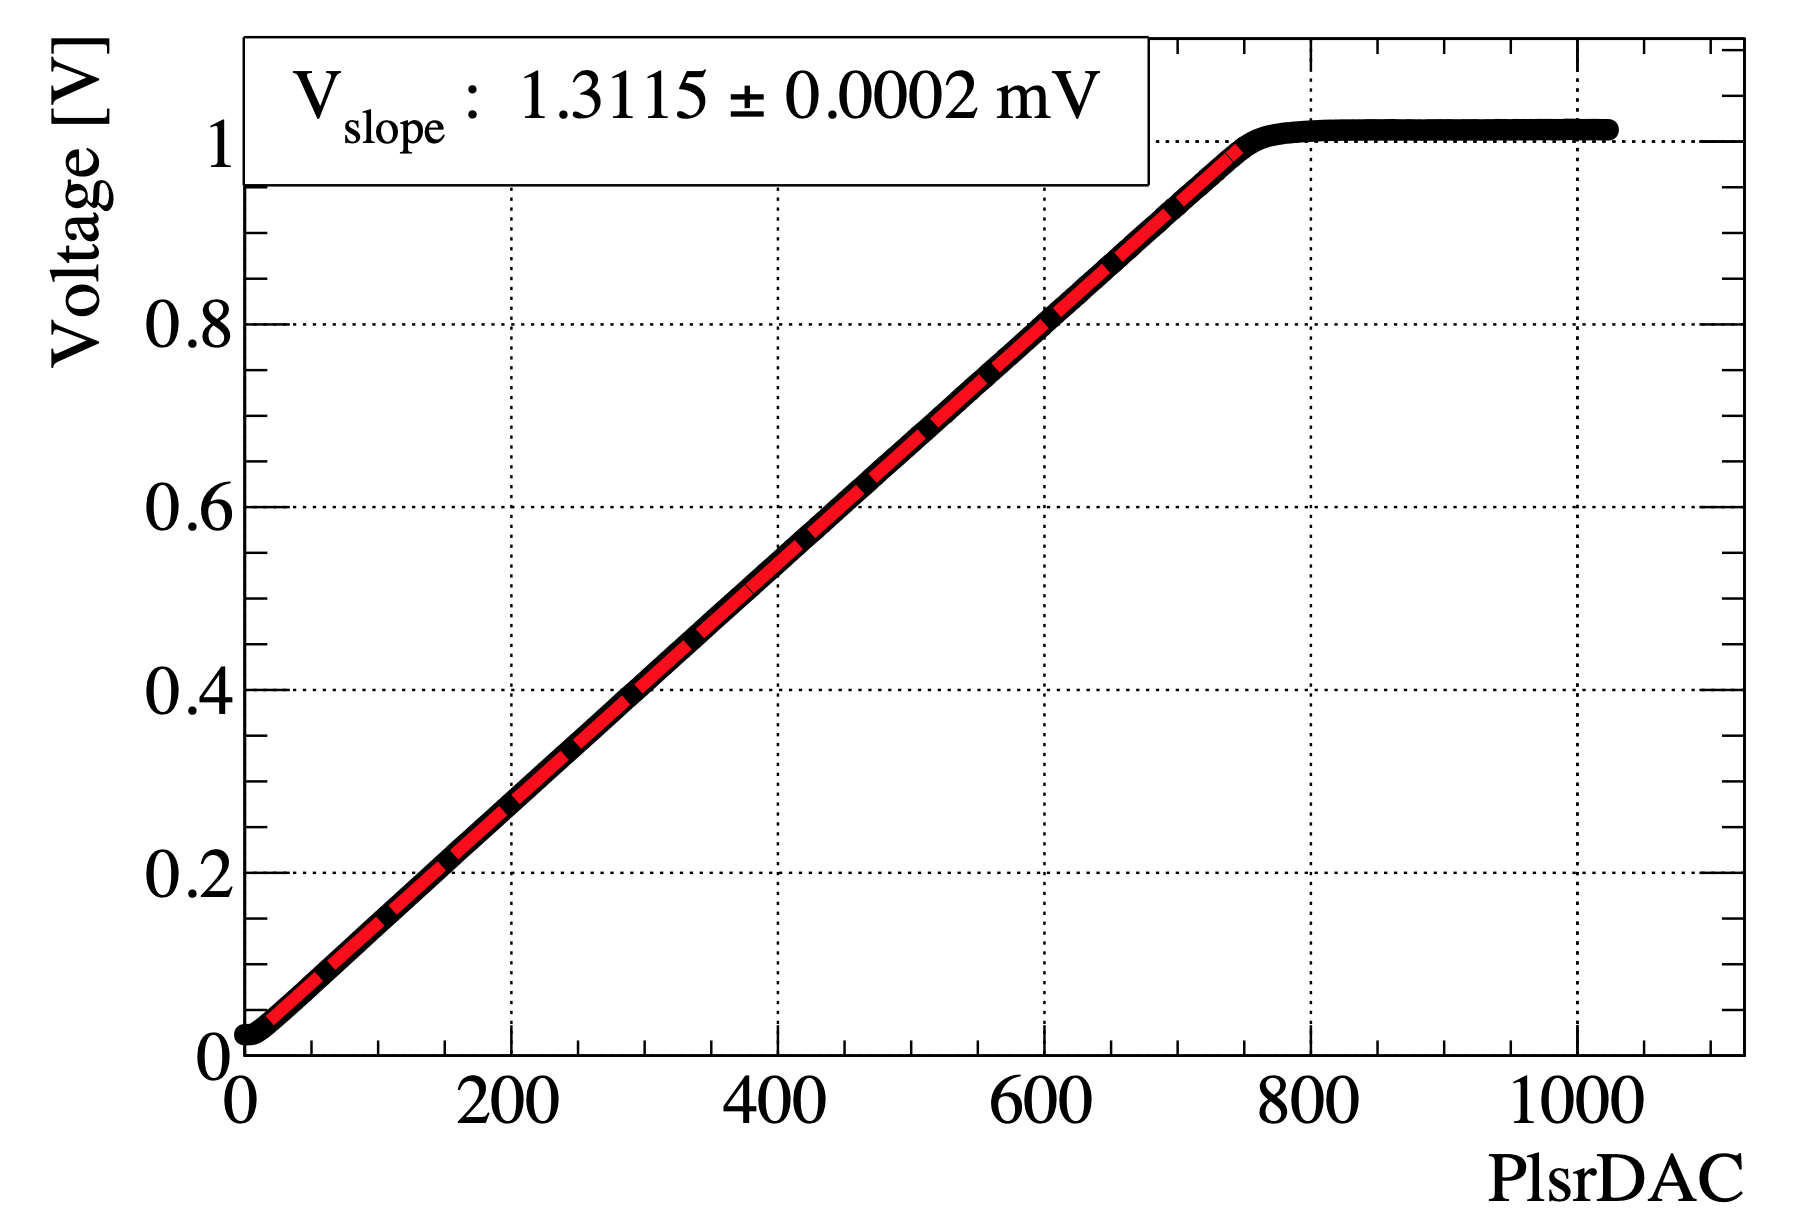
\includegraphics[height=7cm,keepaspectratio]{vcalplsr.png}
  \caption[$V_\mathrm{cal}$とPlsr DACの関係の測定結果]{$V_\mathrm{cal}$とPlsr DACの関係の測定結果 \cite{vcal}。黒点は各Plsr DACに対する$V_\mathrm{cal}$の測定点を表し、赤線は\eref{eq:vcal}を用いたフィッティング結果である。図中における$V_\mathrm{slope}$は赤線の傾きであり、\eref{eq:vcal}における$b$に対応する。}
  \label{fig:vcalplot}
\end{figure}

2つ目の問題に関して、あるFEチップに対してスキャンが失敗してしまった時にデータが欠損してしまうことがある。例えば、Sカーブを用いてThresholdの値を計算するアルゴリズムについて、Sカーブのフィッティングが失敗した際にはThresholdの値がデフォルトで\textbf{0}が出力されるようになっている。そのため、あるFEチップ上の全てのピクセルでSカーブのフィッティングが失敗しているような場合はデータを失い、\fref{fig:thresholdkekkan}のI6が示す領域のようにFEチップ上の全てのピクセルにおいてThresholdの値は$0$を出力する。
このように、あるFEチップについて全てのデータが欠損してしまっている場合には、他の電荷較正結果をコピーすることにより補完を行う。あるピクセルモジュールにおいてFEチップの一部の結果が欠損してしまっている場合は最も近いFEチップから値をコピーすることにより補完を行う。\fref{fig:thresholdkekkan}のようにあるモジュール上の一部のFEチップにデータの欠損が見つかった場合は、最も近いFEチップ(\fref{fig:thresholdkekkan}の場合はI5、I7、I9のいずれか1つ)から値をコピーすることによって補完作業を行う。一方で、あるモジュールについて全てのFEチップの結果が欠損している場合は、直前に行われた電荷較正結果をコピーすることにより補完を行う。

\begin{figure}[tbp]
  \centering
  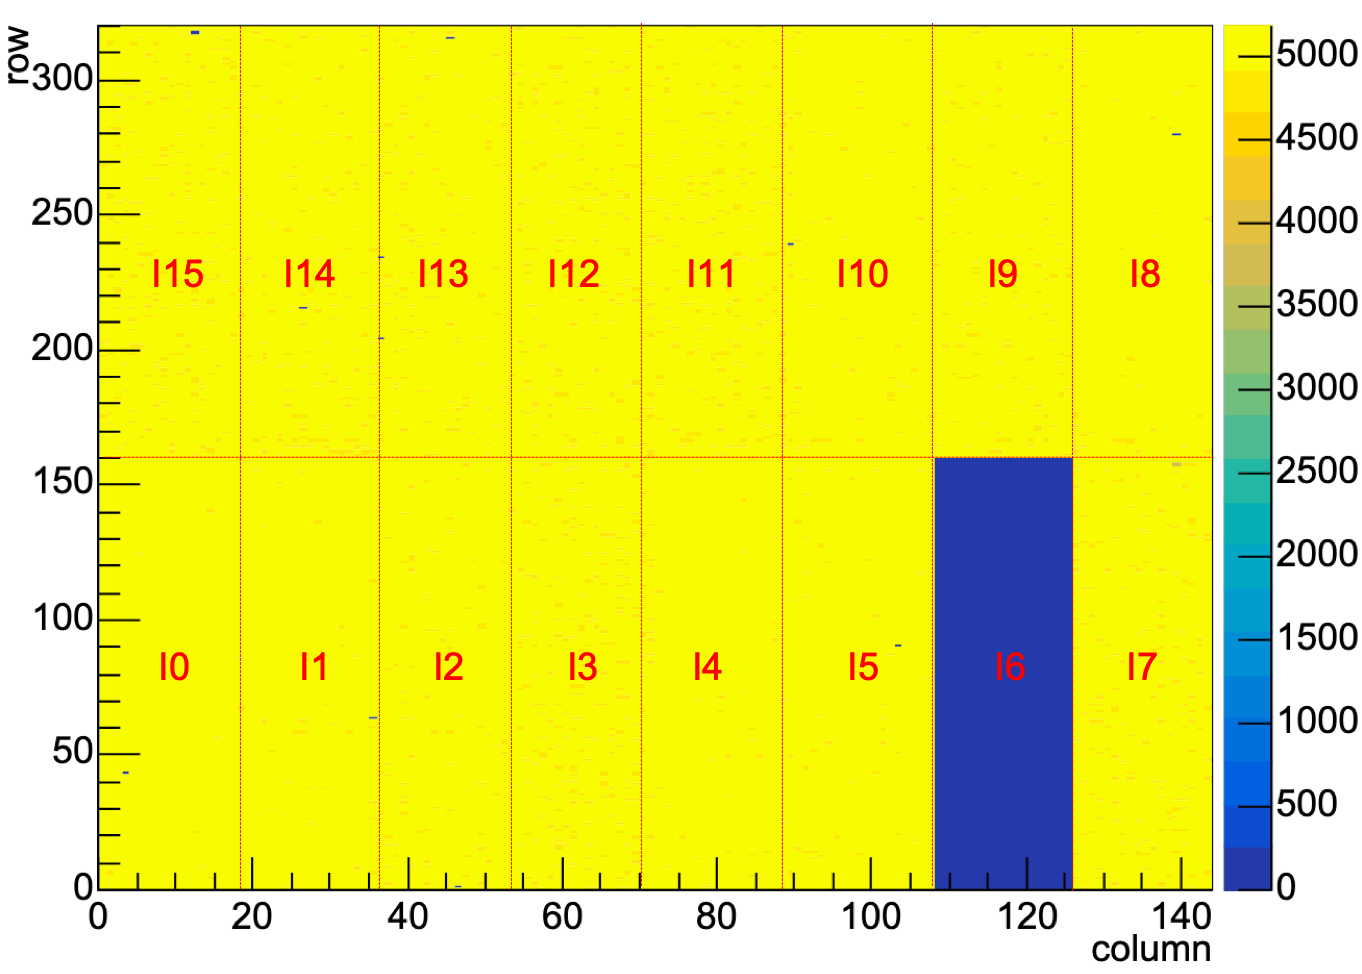
\includegraphics[height=7cm,keepaspectratio]{thresholdkekkan.png}
  \caption[欠損が含まれるピクセルモジュールについてのThreshold分布]{欠損が含まれるピクセルモジュールについてのThreshold分布。赤色の点線は$2\times8$ [行$\times$列]上に配置されたFE-I3の境界部分を表す。この図のように、ThresholdスキャンやToTスキャンの結果はモジュールごとに出力され、行と列の領域を指定することによりFEチップの識別を行うことができる。}
  \label{fig:thresholdkekkan}
\end{figure}

%------------------------------------------------------------------------------------------------------------------------
\subsection{Run2の電荷較正の再補正}
\label{sec:prehosei}
%------------------------------------------------------------------------------------------------------------------------

ATLASに搭載されたピクセル検出器およびIBLのピクセルモジュールについて電荷較正を行うが、測定を行っていると放射線損傷の影響によって、補正値がずれてしまう。\fref{fig:thresholdhennka}にRun2におけるIBLのMIP粒子に対するToTの推移を示す。
このToTの推移はトータルドーズ効果による放射線損傷(\fref{fig:totaldoze}参照)を受けることによるものである。
2015年のRun2序盤における放射線損傷が小さい場合(TID $\leq1\ [\si{Mrad}]$)、放射線損傷によりFEチップ電流は増加する。そのため、実行的なThreshold値が大きくなり、MIP粒子に対するToTは小さくなる(\fref{fig:thresholdhennka}の上図)。
一方で、2018年のRun2終盤における放射線損傷が大きい場合(TID $\geq1\ [\si{Mrad}]$)、放射線損傷によりFEチップ電流は小さくなる。そのため、実行的なThreshold値が小さくなり、ToTの値は大きくなる(\fref{fig:thresholdhennka}の下図)。

%トータルドーズ効果とセンサーの漏れ電流の関係を\fref{fig:totaldoze}示す。

%IBLではMIP粒子がセンサーに落とす電荷量は$16\ \si{ke}$であるが、
このように、放射線損傷を受けることによりToTの値が目標値である$10\ \si{ToT}$から変化していることがわかる。目標値から大きくずれてしまうと、検出器を通過する荷電粒子がセンサーに落とす電荷量を正確に測定できなくなる。さらに、ThresholdやToTの分散も大きくなることから、信号とノイズの分離が悪くなる可能性がある。
目標値からのずれを補正するため、2018年における電荷較正は2週間から4週間の周期で行い、電荷較正の後には\ref{sec:hoseigaiyou}節で説明した問題を取り除くため、補完作業を行う必要がある。

\begin{figure}[tbp]
  \centering
  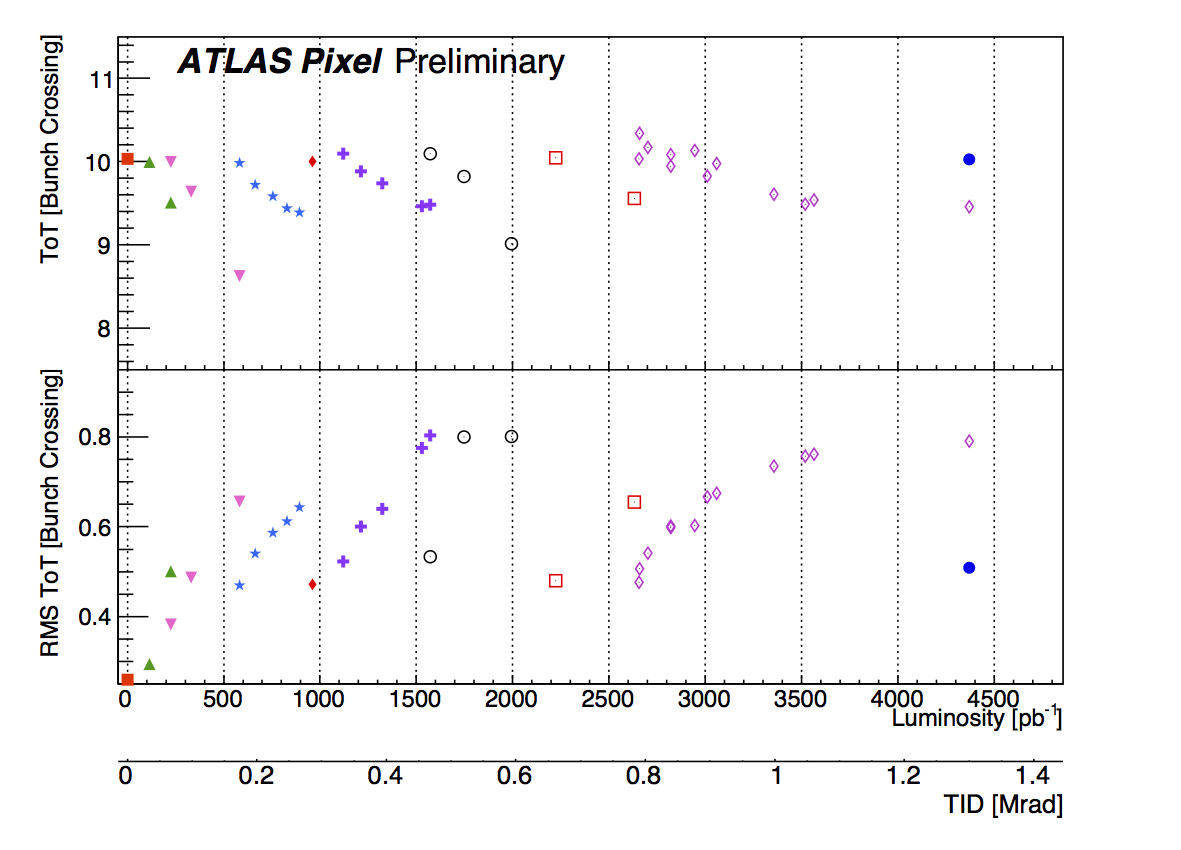
\includegraphics[height=7.8cm,keepaspectratio]{tothennkarow.png}
  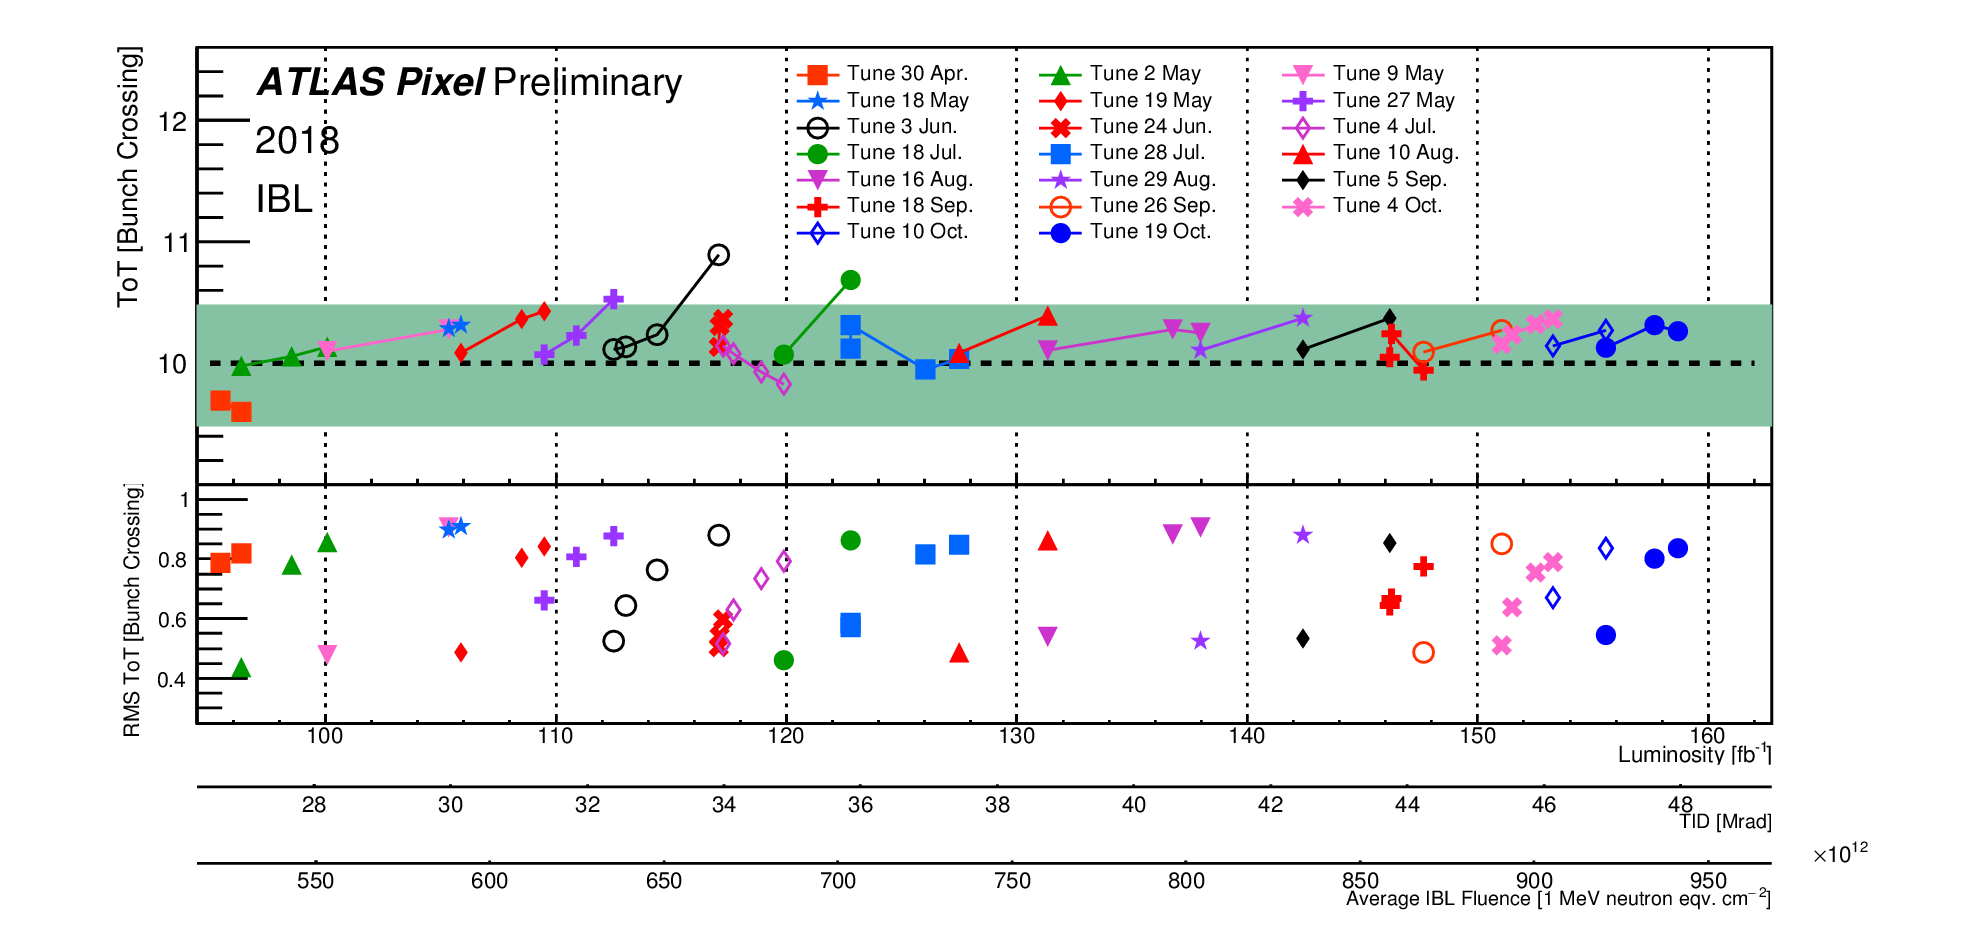
\includegraphics[height=7.5cm,keepaspectratio]{tothennka.png}
  \caption[ルミノシティに対するToTの変化]{IBLのルミノシティに対するToTの変化 。各マーカーの左端は電荷較正直後のToTスキャン結果であり、電荷較正を行う事により放射線損傷によるずれが補正されている様子がわかる。上図は2015年におけるToTの変化\cite{tothenkarow}であり、左端はRun2開始時を表す。下図は2018年におけるToTの変化\cite{tothennka}で右端はRun2の最後を表す。IBLのToTの目標値は$16\ \si{ke}$の電荷量に対して$10\ \si{ToT}$であるが、トータルドーズ効果の影響を受け目標値からずれてしまう。}
  \label{fig:thresholdhennka}
\end{figure}


%\begin{figure}[tbp]
%  \begin{minipage}[b]{0.5\linewidth}
%    \centering
%    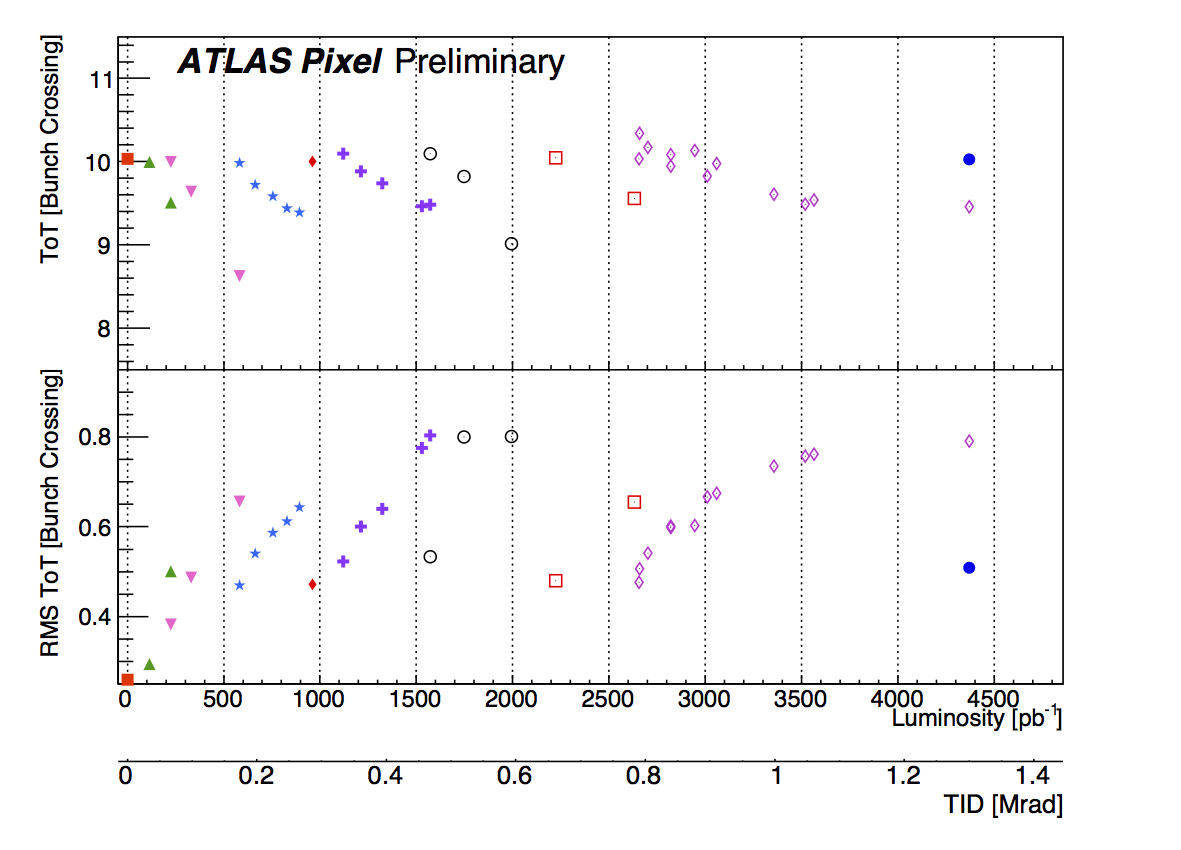
\includegraphics[keepaspectratio, scale=0.4]{tothennkarow.png}
%  \end{minipage}
%  \begin{minipage}[b]{0.5\linewidth}
%    \centering
%    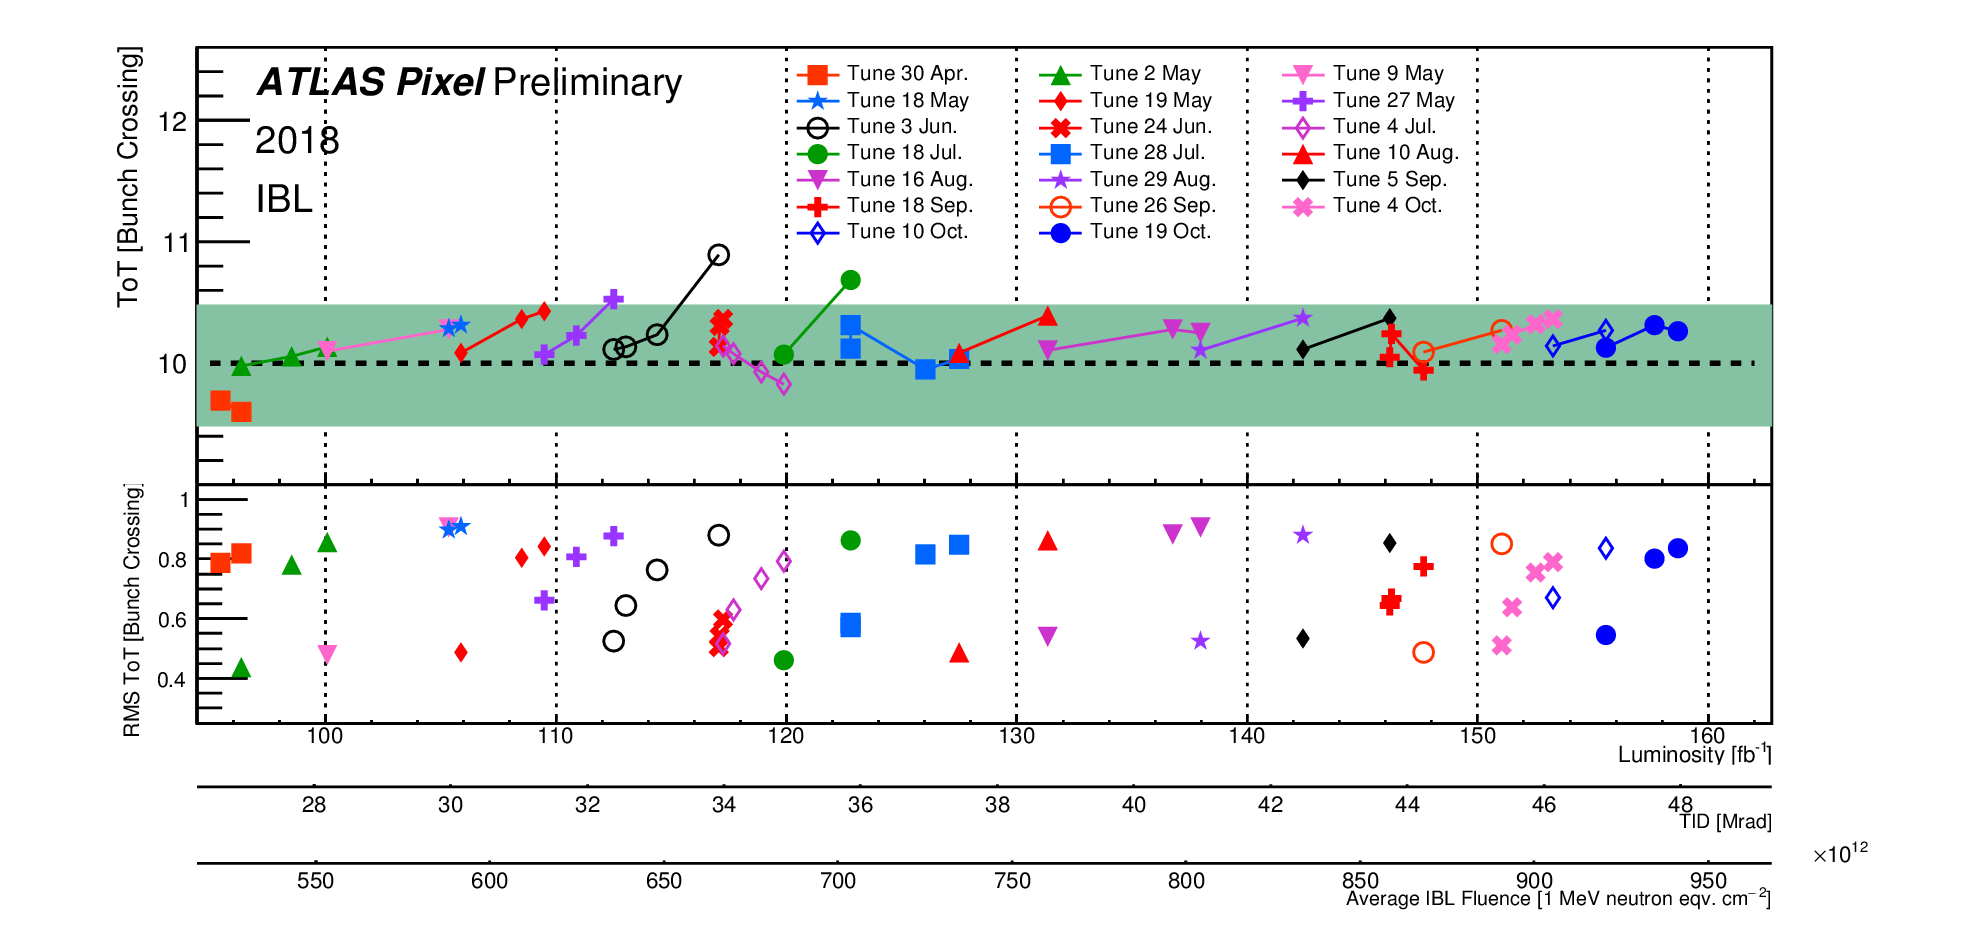
\includegraphics[keepaspectratio, scale=0.2]{tothennka.png}
%  \end{minipage}
%  \caption[ルミノシティに対するToTの変化]{ルミノシティに対するToTの変化}
%  \label{fig:calibhikaku}
%\end{figure}

%\begin{figure}[tbp]
%  \centering
%  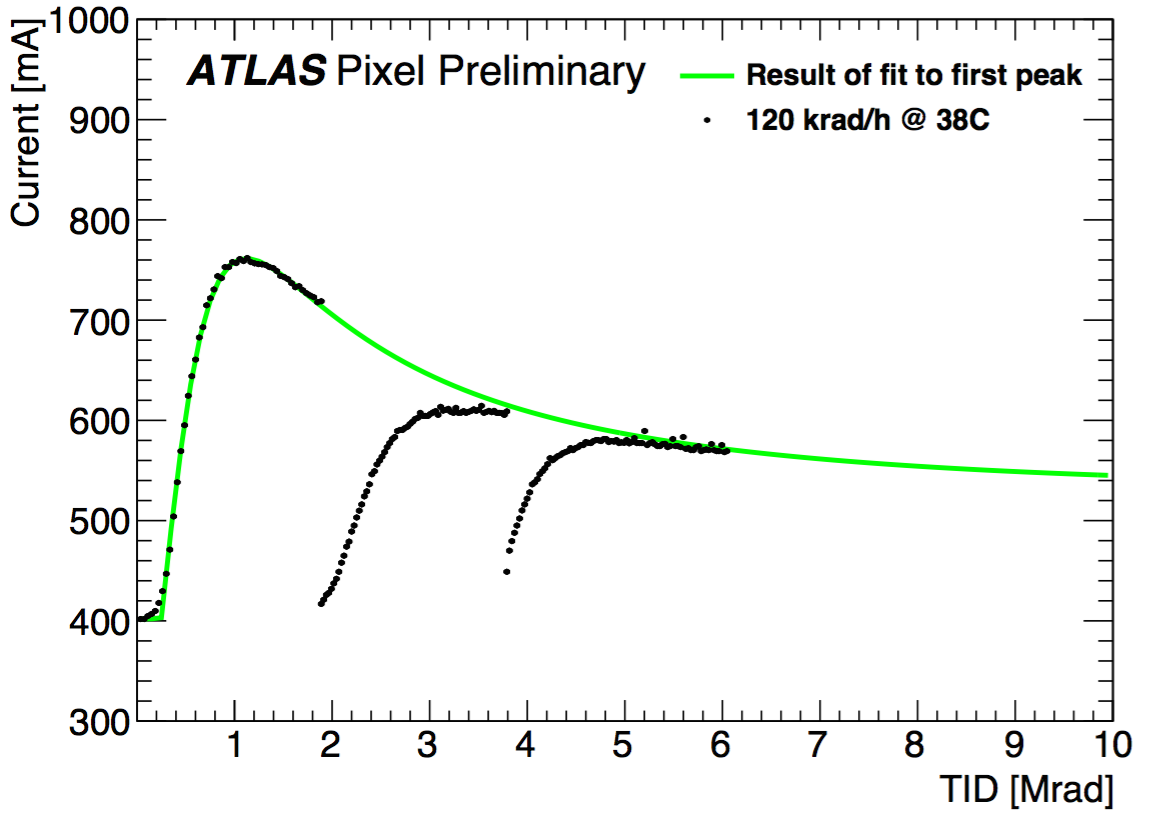
\includegraphics[height=7.5cm,keepaspectratio]{totaldose.png}
%  \caption[トータルドーズ効果と漏れ電流の関係]{トータルドーズ効果と漏れ電流の関係 \cite{totaldoze}。}
%  \label{fig:totaldoze}
%\end{figure}


これまで、電荷較正後の補完作業は1人の担当者による手作業で行われていた。Run3からは放射線損傷による影響がさらに大きくなることから、電荷較正の頻度が10日に1度程度になる予定であり、この作業を行うのは非常な労力が伴う。さらに、これまで行っていた補正では手作業による補正であることから、担当者によっては異なる値を補完してしまうことがある。本研究では適切な欠損の補完処理を行うよう、例外をアルゴリズムとして抽出・処理する自動解析ツールの開発を行った。次節からその詳細について説明する。


%------------------------------------------------------------------------------------------------------------------------
\section{電荷較正の補正}
\label{sec:calibhosei}
%------------------------------------------------------------------------------------------------------------------------
\fref{fig:calibhikaku}の右図に示すように、電荷生成のための回路の個体差により正しい電荷が生成できず、誤ったToTを持つ電荷を用いて電荷較正を行ってしまう場合がある。この様な点を取り除くために、これまでは\eref{eq:averagedistance}を用いて電荷較正結果の評価を行っていた。
\begin{equation}
  \label{eq:averagedistance}
  \Delta d = \sum_{i=1}^{N} \frac{|ToT_{true, i} - ToT_{fit, i}|}{N}
\end{equation}
ここで、$N$は電荷較正に使われた試験電荷の数であり、$ToT_{true, i}$および$ToT_{fit, i}$はそれぞれ電荷較正に使用された試験電荷の$i$番目のToT、電荷較正式によるフィッティングから得られる$i$番目のToTである。つまり、$\Delta d$は試験電荷から得られるToTとフィッティングから得られる得られるToTの絶対差の平均値を計算している。
%電荷較正結果の評価のために、全てのFEチップにおいて計算した$\Delta d$の分布を\fref{fig:averagedistance}に示す。
この評価では$\Delta d > 0.5$の場合、電荷較正に正しく生成されいない試験電荷が存在するとし、そのフィッティング結果を取り出して補正を行う。2018年9月における電荷較正では、約250個の正しく電荷が生成されていないフィッティング結果が見つかり、その補正を行った。

%\begin{figure}[tbp]
 % \centering
 % 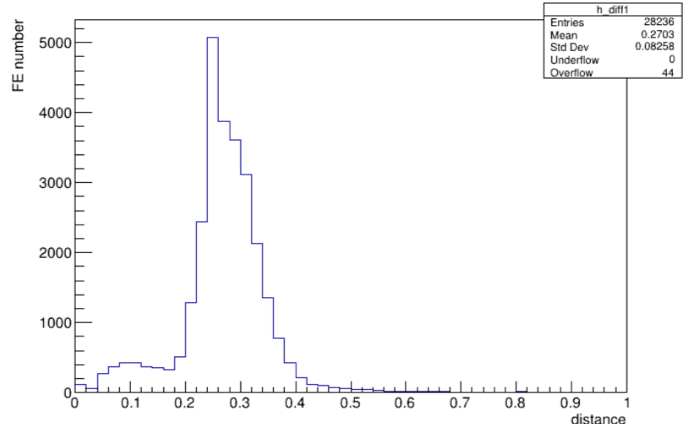
\includegraphics[height=6cm,keepaspectratio]{averagedistance.png}
 % \caption[電荷較正結果の評価のための$\Delta d$の分布]{電荷較正結果の評価のための$\Delta d$の分布。}
%  \label{fig:averagedistance}
%\end{figure}

電荷較正は一部のデータ点にのみ問題が含まれると予想されるため、\eref{eq:averagedistance}の評価方法は電荷較正に使う試験電荷の数によって大きさが変化するものである。そのため、問題のある試験電荷を取り除いた後の電荷較正結果の評価のための基準値は、$0.5$とは別の値を用いる必要がある。しかし自動補正を行う際、電荷再較正を行う度に基準値を変更するのは非常に困難である。
そこで、本研究で新たな評価基準を導入し、それを用いた電荷再較正の自動化アルゴリズムの開発を行った。


%------------------------------------------------------------------------------------------------------------------------
\subsection{電荷較正結果の評価方法}
%------------------------------------------------------------------------------------------------------------------------
電荷較正結果を評価するための新たな基準を以下に示す。
\begin{screen}
電荷較正データの試験電荷量と\eref{eq:calibration}のフィット結果から得られる電荷量の差が、試験電荷量の5\%以上であれば問題のある試験電荷とみなす
\end{screen}
上記の評価基準は、ピクセル検出器における主な測定対象であるMIP粒子の検出感度から決定した。MIP粒子がピクセル検出器に落とす電荷量の分布を\fref{fig:mipdist}に示す。荷電粒子がシリコンセンサーに落とす電荷の分布はLandau分布に従う。MIP粒子がシリコンセンサーに落とす電荷量の測定分解能は$15\%$程度である。上記の基準を満たしていれば、電荷較正により得られる電荷量の揺らぎを\fref{fig:mipdist}におけるランダウ分布の揺らぎより十分小さく抑制することができる。

\begin{figure}[tbp]
  \centering
  \includegraphics[height=7cm,keepaspectratio]{mipdist.png}
  \caption[MIP粒子がピクセル検出器に落とす電荷量]{ピクセル検出器の$250\ \si{\micro m}$あたりのピクセル検出器にMIP粒子が落とす電荷量。現行ピクセル検出器におけるセンサーの厚みは$250\ \si{\micro m}$のため、MIP粒子が落とす電荷量に相当する。クラスターはnormalピクセルのみからつくられるものであり、ピクセルの短方向($50\times400\ \si{\micro m^2}$[行$\times$列]の$50\ \si{\micro m}$の方向)に2つピクセルから構成されるクラスターのみのデータである。}
  \label{fig:mipdist}
\end{figure}

%上記の基準を満たしていれば、MIP粒子がシリコンセンサーに落とす電荷の測定精度$5\%$であり、電荷較正による分解能が\fref{fig:mipdist}におけるランダウ分布の揺らぎより十分小さくできる。

また、この基準は各試験電荷について個別の評価を行っているため、試験電荷の数に依存せず電荷再較正の自動処理により適した評価方法である。\fref{fig:partialdistance}にB-Layerの全FEチップについて計算した試験電荷と電荷較正結果から得られる電荷の差の分布を示す。この分布において、試験電荷とから得られる電荷の差と試験電荷の比が$5\% $より大きいFEチップについて電荷較正結果の補正を行う。次項において、電荷再較正の処理方法について説明する。

\begin{figure}[tbp]
  \centering
  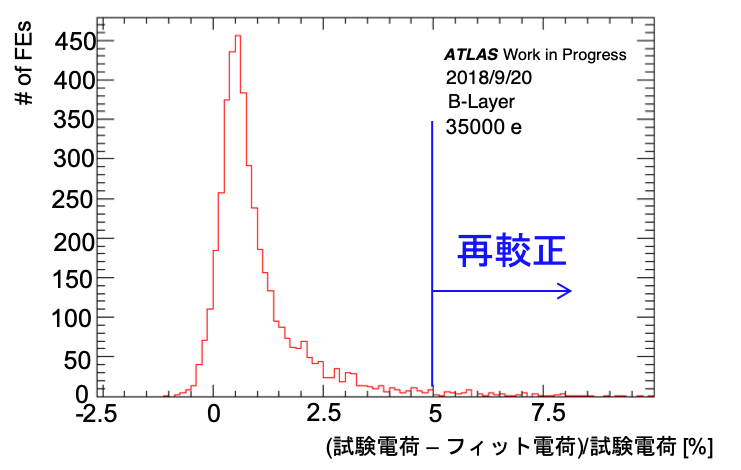
\includegraphics[height=7cm,keepaspectratio]{partialdistance.png}
  \caption[B-Layerの全FEチップについて計算した試験電荷と電荷較正結果から得られる電荷の差の分布]{B-Layerの全FEチップについて計算した試験電荷と電荷較正結果から得られる電荷の差の分布。この図は試験電荷量$35000\ \si{e}$とその試験電荷に相当するToTを用いてフィット関数\eref{eq:calibration}から逆算される電荷量の差の相対比の分布を表す。}
  \label{fig:partialdistance}
\end{figure}


%------------------------------------------------------------------------------------------------------------------------
\subsection{電荷再較正の自動化アルゴリズム}
%------------------------------------------------------------------------------------------------------------------------
上記の評価基準を用いて電荷再較正を自動で行うツールを作成した。解析処理を行うために、CERNが提供している解析フレームワークであるROOTを使用している。電荷較正のために作成されたROOTの解析ツールを改良し、電荷較正後に結果の評価および再較正を行うプログラムを追加した。
作成したツールの処理の流れを\fref{fig:saikouseiflow}に示す。

\begin{figure}[tbp]
  \centering
  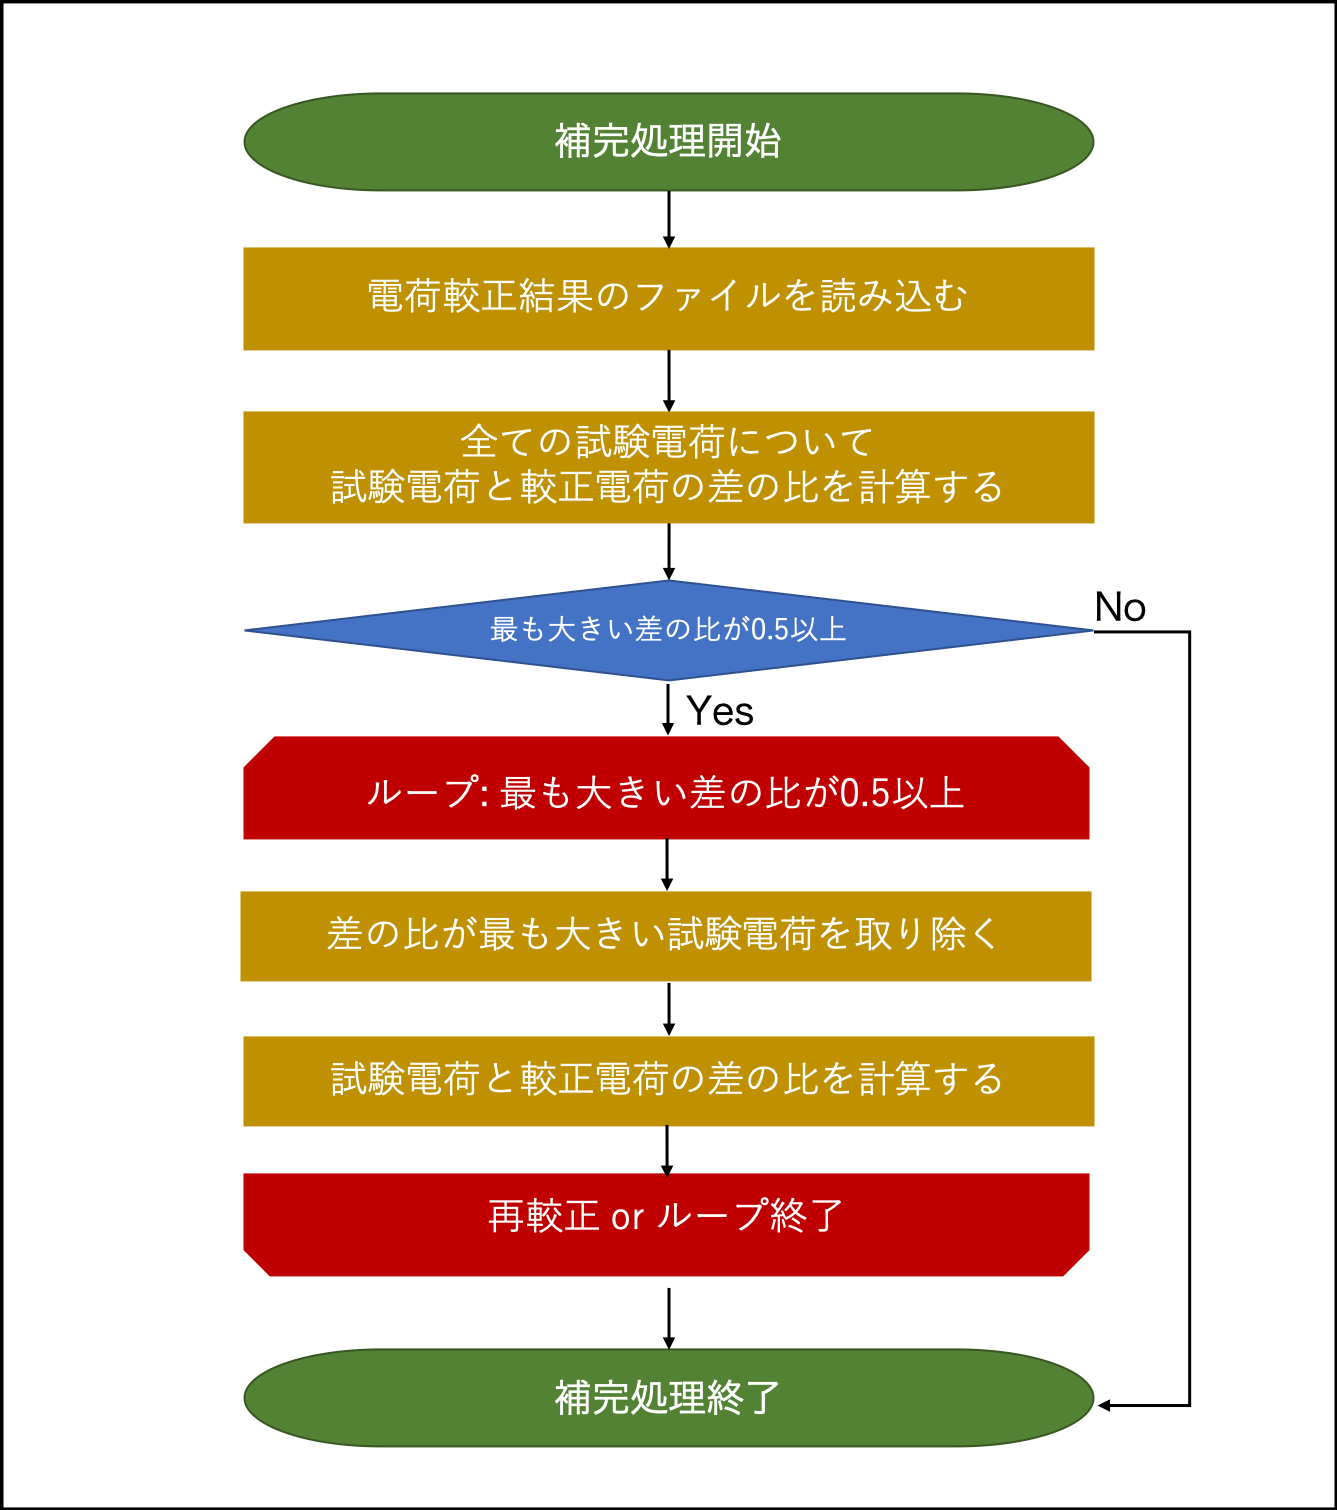
\includegraphics[height=10cm,keepaspectratio]{saikouseiflow.png}
  \caption[電荷較正結果を再較正するツールの処理の流れ]{電荷較正結果を再較正するツールの処理の流れ。}
  \label{fig:saikouseiflow}
\end{figure}


\fref{fig:saikouseiflow}に示したループの処理で電荷較正から得られる電荷と試験電荷の差の相対比が$5\%$以内に収束するまで再較正の処理を行う。これにより問題のある試験電荷を全て取り除いて電荷較正を行うことができる。電荷再較正のアルゴリズムを用いて問題のある試験電荷を取り除き再構成した結果を\fref{fig:calibhosei}に示す。この場合、始めのループで$35000\ \si{e}$の試験電荷を取り除き、次のループで$30000\ \si{e}$が取り除かれる。それにより、電荷較正から得られる電荷と試験電荷の差の相対比が$5\%$以内に収束し、正しい電荷再較正結果が得られる。

\begin{figure}[tbp]
  \begin{minipage}[b]{0.5\linewidth}
    \centering
    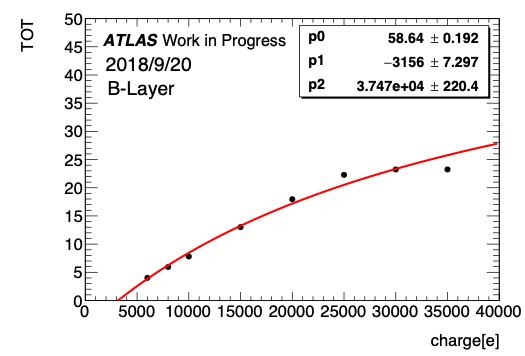
\includegraphics[keepaspectratio, scale=0.85]{calibhoseimae.png}
  \end{minipage}
  \begin{minipage}[b]{0.5\linewidth}
    \centering
    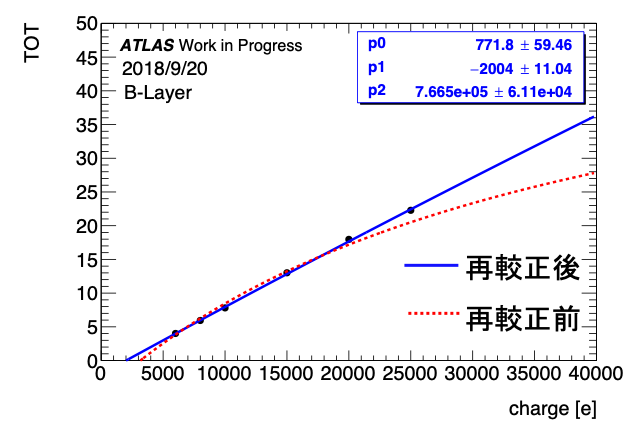
\includegraphics[keepaspectratio, scale=0.72]{calibhoseigo.png}
  \end{minipage}
  \caption[電荷再較正前後のフィッティング結果]{電荷再較正前(左図)と後(右図)のフィッティング結果。}
  \label{fig:calibhosei}
\end{figure}


%------------------------------------------------------------------------------------------------------------------------
\section{データに欠損が含まれる場合の補完}
\label{sec:kessonhosei}
%------------------------------------------------------------------------------------------------------------------------
これまではピクセルモジュール内の一部のFEチップに欠損しているデータがある場合には、最も近いFEチップから値をコピーすることにより補完していた。しかし、現行のピクセル検出器(IBLを除く)におけるモジュールは近いFEチップは2つまたは3つあるため、どの値を用いて補完を行うかは担当者の裁量によるものであった。結果を一意に決定するために、適切な自動処理を行う必要がある。より適切な方法を用いて自動処理を行うために、以下の二つの補完方法を導入する。
\begin{itemize}
  \item[1. ] 同一FEチップ上の他のピクセルタイプの平均値を用いた補完(\fref{fig:houhouhou}の左)
  \item[2. ] 欠損している部分を除いた全てのFEチップの平均値を用いた補完(\fref{fig:houhouhou}の右)
\end{itemize}
各パラメータの補完のため、2つの補完方法の内、どちらがより実際の値を再現するかの評価を行った。

\begin{figure}[tbp]
  \begin{minipage}[b]{0.45\linewidth}
    \centering
    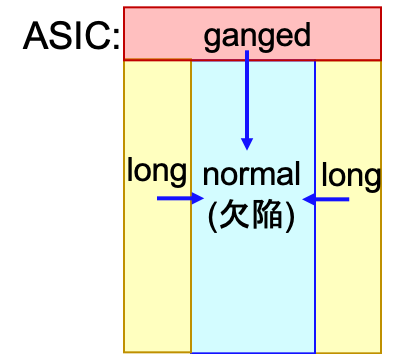
\includegraphics[keepaspectratio, scale=0.6]{houhousame.png}
  \end{minipage}
  \begin{minipage}[b]{0.55\linewidth}
    \centering
    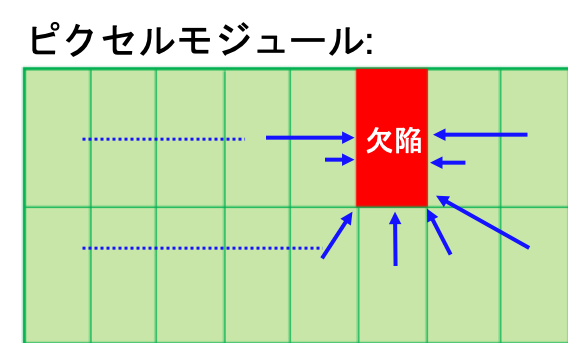
\includegraphics[keepaspectratio, scale=0.7]{houhoudiff.png}
  \end{minipage}
  \caption[データ欠損の補完方法]{データ欠損の補完方法についての概念図。それぞれの図は"欠損"と書かれている部分のデータが欠けており、青矢印のように補完している。左図は1つのFEチップを表し、normalピクセルの値が欠損している場合に、longおよびgangedピクセルの平均値を用いて補完する様子を示す。右図は1つのピクセルモジュールを表し、赤色の部分におけるFEチップの値が欠陥している場合に、異なるFEチップの平均値を用いて補完する様子を示す。}
  \label{fig:houhouhou}
\end{figure}


%------------------------------------------------------------------------------------------------------------------------
\subsection{評価方法}
%------------------------------------------------------------------------------------------------------------------------
補完方法の評価のため、電荷較正結果に含まれるパラメータの1つが欠損していると仮定し、そのパラメータと補完により得られる値の差を計算し分布の作成を行った。評価を行う際、2018年9月に行われた電荷較正の結果を用いた。IBLおよびピクセル検出器の全ての層について評価を行ったが、全ての層について同様の結果が得られたため、以下ではB-Layerの結果のみについての議論を行う。

%------------------------------------------------------------------------------------------------------------------------
\subsection{評価結果と考察}
%------------------------------------------------------------------------------------------------------------------------

前節において説明した方法を用いて、補完方法の評価を行った。\fref{fig:kekkanthreshold}はNormalピクセルにおけるThresholdについての評価結果を表す。この結果から、 \underline{Threshold値は補完方法1の同一FEチップにお}\\ \underline{ける別のピクセルタイプから得られる平均値を用いて補完}した場合の方が、より精度良く補完を行うことがわかる。これはThresholdのチューニング方法によるものだと考えられる。チューニングではあるFEチップにおけるピクセル全体にGlobalチューニングを行った後、各ピクセルごとにLocalチューニングを行う。初めにGlobalチューニングを行うことから、別のFEチップの値を用いて補完するより、同一FEチップの値を用いて補完する方が実際の値に近い値を用いた補完を行うことができる。

\fref{fig:kekkannoise}はNormalピクセルにおけるThresholdのノイズについての評価結果を表す。この結果から、\underline{ノイズは補完方法2の別のFEチップにおける同一ピクセルタイプから得られる平均値を用いて補完}した場合の方が、より精度良く補完を行うことができるとわかる。GangedピクセルはNormalピクセル2つをワイヤーで接続しているため、Normalピクセルに比べてノイズが大きくなる。さらに、Longピクセルは長方形の長辺の長さがNormalピクセルの1.5倍あるため、Normalピクセルと比べてピクセル間に生じるキャパシタンスが大きくなる。これによりFEチップ内の回路にノイズが加わり、LongピクセルのノイズはNormalピクセルよりもノイズが大きくなる。


\begin{figure}[tbp]
  \begin{minipage}[b]{0.5\linewidth}
    \centering
    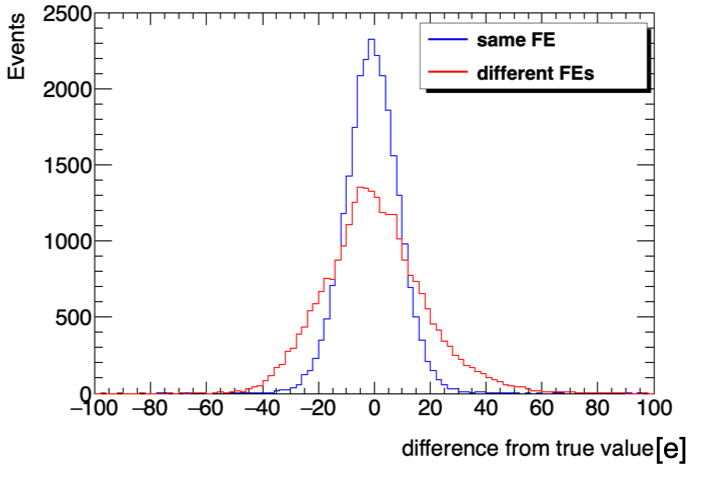
\includegraphics[keepaspectratio, scale=0.6]{kekkanthreshold.png}
    \caption[Thresholdの評価結果]{Thresholdの評価結果。同一FEチップにおける平均値の分布(青色)は、異なるFEチップの値の平均値の分布(赤色)よりのピークが鋭くなっている。}
    \label{fig:kekkanthreshold}
  \end{minipage}
  \begin{minipage}[b]{0.5\linewidth}
    \centering
    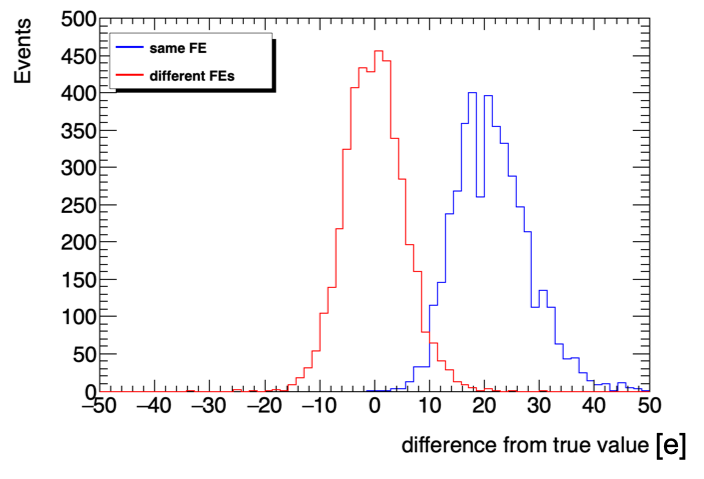
\includegraphics[keepaspectratio, scale=0.6]{kekkannoise.png}
    \caption[Thresholdのノイズの評価結果]{Thresholdのノイズの評価結果。同一FEチップの平均値の分布(青色)は、ピークの中心値がゼロからずれている。\\}
    \label{fig:kekkannoise}
  \end{minipage}
\end{figure}

他のパラメータについては\fref{fig:kekkannoise}と同様に、補完方法1と2の分布のピークの中心値が異なる結果が得られたため、補完方法2を用いることにより実際の値に近い値を再現できると考えられる。

%------------------------------------------------------------------------------------------------------------------------
\subsection{欠損補完のための解析ツール}
%------------------------------------------------------------------------------------------------------------------------
上記の評価結果を用いて、自動で補完処理を行うツールの作成を行った。欠損補完のための処理の流れを以下に示す。
\begin{itemize}
  \item[1. ] 補完結果のファイルを読み込む
  \item[2. ] 結果ファイル内の全てのモジュールについて、補完方法1および2を用いて値の補完を行う
  \item[3. ] スキャンが行われていないモジュールがあれば、一つ前の電荷較正結果の値をコピーし補完する
  \item[4. ] 補完結果をデータベースにアップロード可能なフォーマットに整形する
\end{itemize}

電荷較正結果をデータベースにアップロードするためには、電荷較正が行われていないモジュールの結果についても結果ファイル内に書き込む必要がある。そのため、処理の流れの3のように、電荷較正が行われていないモジュールについては1つ前の電荷較正結果から値をコピーすることにより補完を行う。また、データベースへアップロードするためには補完結果のファイルの中身を整形する必要があり、その処理についても補完処理を行うツールの最後に行う。

%------------------------------------------------------------------------------------------------------------------------
\section{自動補完のための解析ツール}
\label{sec:kaisekitool}
%------------------------------------------------------------------------------------------------------------------------
\ref{sec:calibhosei}節および\ref{sec:kessonhosei}節で示した補完方法を用いて自動で補完処理を行う解析ツールの開発を行った。解析ツールが行う処理の流れを以下に示す。

\begin{itemize}
  \item[1. ] \fref{fig:saikouseiflow}の流れで電荷較正および再較正
  \item[2. ] CERNのデータベースにアクセスし、1つ前の電荷較正結果の履歴を取得
  \item[3. ] \ref{sec:kessonhosei}節に示した解析ツールを用いて欠損の補完および結果ファイルの整形
  \item[4. ] 補完についてのまとめファイルを出力
\end{itemize}

処理の流れの4番目に示すように、電荷再較正および欠損の補完を行った後にどのような補完を行ったかについてのまとめファイルを出力する。まとめファイルの例を\cref{code:matomefile}に示す。まとめファイルのはじめに、どのように補完が行われるかを記し、その後に補完結果が確認できるようにした。

\begin{lstlisting}[caption=解析ツールにより出力される補完結果のまとめ。,label=code:matomefile, language=C++]
##===========================================================================
## This file shows the way to recover data loss and calibration failure.
##
## How to recover parameters:
## 1. If there is a data loss in output data:
##   - Case1: Partial loss in a module
##     - Threshold: Recover using average of same FE
##     - Others:    Recover using average of different FEs
##   - Case2: All values loss in a module
##     - Previous scan result is used for the recovery
##
## 2. If there is a calibration failure:
##   - Remove incorrect injected charge & refitting
##   - Removed charges are listed in order of deletion
##
## Example of an output for a module:
##   L0_B08_S1_A6_M2A:
##   I2: [ normal threshold ], [ ] <--- Parameters that become '0' is listed
##   I8: [ ], [ 30000 40000 ] <-------- Injected charges that removed is listed
##
##===========================================================================

~~~~~~~~ Summary for the recovery ~~~~~~~~
1. Number of parameters that were 0
Number of FEs with all values zero: 11
normal threshold: 11
normal noise: 11
normal sigma: 11
normal intime: 27
fit_normal A: 11
fit_normal E: 11
fit_normal C: 11
quality/unused unused: 11
quality/unused fit_quality: 11

2. Number of FEs that had bad fits
B-Layer: 0
Layer1: 0
Layer2: 0
Disk: 5

3. Number of modules that were not scanned
B-Layer: 286
Layer1: 494
Layer2: 676
Disk: 6
~~~~~~~~~~~~~~~~~~~~~~~~~~~~~~~~~~~~~~~~~~

D1A_B01_S1_M1:
I0 [ normal threshold ], [ ]
D1A_B01_S1_M2:
D1A_B01_S1_M3:
I8: [ ], [ 30000, 40000 ]
\end{lstlisting}



%------------------------------------------------------------------------------------------------------------------------
\section{解析ツールの運用}
\label{sec:unnyou}
%------------------------------------------------------------------------------------------------------------------------

Run3におけるATLAS実験のためのモンテカルロシミュレーションのサンプル作成のために、2021年9月に電荷較正のためのデータ取得が行われた。電荷較正結果をデータベースにアップロードするために、本研究で作成した解析ツールを用いて電荷較正結果を作成した。以下では、電荷較正における補完結果をまとめる。


%------------------------------------------------------------------------------------------------------------------------
\subsection{補完のまとめ}
\label{sec:matome}
%------------------------------------------------------------------------------------------------------------------------
電荷較正結果と同時に出力されるファイルを用いて、補完内容の確認を行なった。\tref{tab:hokannmatome}に補完結果のまとめを示す。この結果から、各モジュールに存在した欠損を取り除き、値の再現ができたと考えられる。表中に示すように、B-Layerにおける再較正を行ったFEチップの数は他の層と比較して非常に多くなった。これについて次節にて説明する。

\begin{table}[tbp]
  \begin{center}
    \caption[RUN3に向けた電荷較正補完のまとめ]{RUN3に向けた電荷較正補完のまとめ。次節に示すように、電荷較正および再較正はデータ取得に大きく影響を与えると考えられる電荷量の領域($>5000\ \si{e}$)のみを用いて行った。}
    \label{tab:hokannmatome}
    \begin{tabular}{|l||c|c|c|c|}
    \hline
      補完項目 & B-Layer & Layer1 & Layer2 & Disk  \\
    \bhline{1.5pt}
      スキャンされなかったモジュール数  & 14 & 18 & 40 & 6 \\
    \hline
      欠損していたFEチップの数  & 18 & 46 & 38 & 11 \\
    \hline
      部分的に0となっていたパラメータ数  & 0 & 6 & 8 & 3 \\
    \hline
      再較正を行なったFEチップの数 & 179 & 1 & 9 & 5 \\
    \hline
    \end{tabular}
  \end{center}
\end{table}


%------------------------------------------------------------------------------------------------------------------------
\subsection{Run3に向けた電荷較正結果の再較正}
\label{sec:saisinsaikousei}
%------------------------------------------------------------------------------------------------------------------------

2021年9月に行われた電荷較正で用いた試験電荷の最小値は$3000\ \si{e}$であり、$10000\ \si{e}$までは$500\ \si{e}$ずつ電荷量を変更させてToTスキャンを行い、それ以降は$12000,\ 14000,\ 16000,\ 18000,\ 20000,\ 25000\ \si{e}$の試験電荷を用いてToTスキャンを行う。全ての試験電荷を用いて電荷較正およびその再較正を行った結果を\fref{fig:blayerba}に示す。左図は全ての点を用いて電荷較正を行った結果であり、右図はその再較正結果である。再較正では$5000\ \si{e}$以下の試験電荷を全て取り除くことにより再較正が完了する。

\begin{figure}[tbp]
  \begin{minipage}[b]{0.5\linewidth}
    \centering
    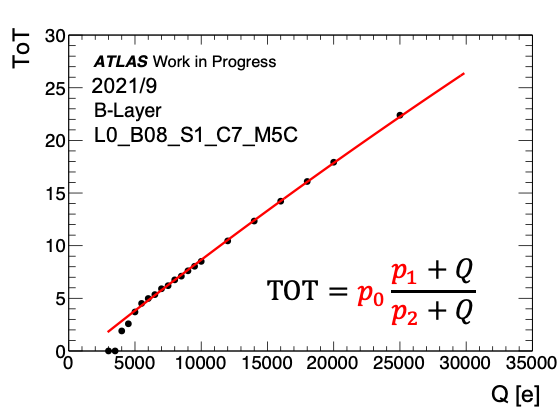
\includegraphics[keepaspectratio, scale=0.8]{blayerbefore.png}
  \end{minipage}
  \begin{minipage}[b]{0.5\linewidth}
    \centering
    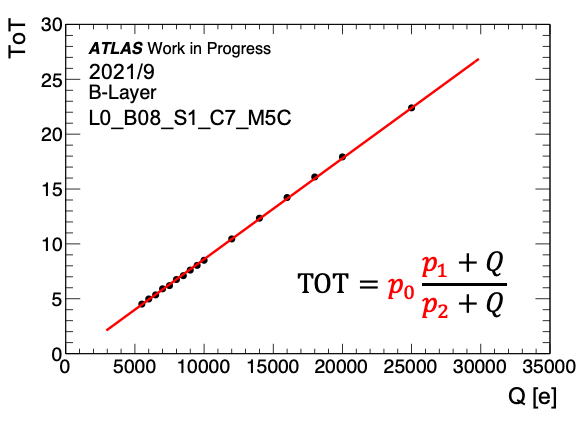
\includegraphics[keepaspectratio, scale=0.78]{blayerafter.png}
  \end{minipage}
  \caption[2021年9月に行われたB-Layerについての電荷較正結果]{2021年9月に行われたB-Layerについての電荷再較正結果。左図は再較正前のフィット結果であり、右図は基準を満たさない点を取り除き再較正を行った後の結果である。}
  \label{fig:blayerba}
\end{figure}

この電荷較正におけるThresholdの値は$3500\ \si{e}$であり、タイムウォーク(\ref{sec:ASIC}節参照)が$25\ \si{ns}$となる電荷量は$5000\ \si{e}$程度である。そのため、$5000\ \si{e}$以下の点はタイムウォークの影響が大きくなることから、本来予想されるToTよりも小さいToTを出力してしまうと考えられる。電荷較正\eref{eq:calibration}は二次的な効果も含めた較正式であるが、このような効果を完全に再現できずにフィット結果がデータ点からずれてしまうと考えられる。

Run2までの電荷較正ではThresholdに近い電荷量を持つ試験電荷について$2000\ \si{e}$ずつ電荷量を変化させていたが、Run3に向けた電荷較正では$500\ \si{e}$ずつ電荷量を変化させ、ToTスキャンを行った。その結果、Threshold付近のToTと電荷量の関係がよく見えるようになり、小さい電荷量を持つ点を除く電荷再較正を行うようになった。この電荷再較正は全てのFEチップにおいて行われるため、補正結果のまとめファイルでは全てのFEチップに正しくない電荷が含まれるという出力が得られた。しかし、全てのFEチップに正しくないという結果は、\fref{fig:calibhosei}のような大きい電荷量でToTが飽和するような問題等をまとめファイルから見つけることが困難になってしまう。そこで、特出して悪い試験電荷が含まれる電荷較正結果のみを抽出できるように$5000\ \si{e}$より大きいの試験電荷のみを用いて電荷較正を行った。その結果のまとめが\tref{tab:hokannmatome}である。
%そこで、データ取得に大きく影響を与えると考えられる電荷量の領域を制限し電荷較正を行った。

%ピクセル検出器におけるデータ取得では、アナログ回路におけるThresholdとは別にToTの閾値を定義することによりヒット情報の記録を行う。ToTの閾値を超える信号を中心にクラスタリングを行い、そのクラスターにおける電荷量の測定やヒットの位置情報を測定する。Run3における電荷較正でのThresholdの値、ToTの閾値およびMIP粒子に相当するToTの値を\tref{tab:run3tuning}に示す。B-LayerにおいてはToTの閾値が$3$であり、ToTが$4$以上のヒットを用いてクラスタリングが行われる。そのため、$4\ \mathrm{ToT}$に相当する電荷量である$5000\ \si{e}$以上の試験電荷を用いて電荷較正を行った。また、他の層についてもB-Layerと同様の範囲を用いて電荷構成を行った。この試験電荷の範囲を用いて電荷較正結果の再較正を行った数が\tref{tab:hokannmatome}に記されている。

\begin{table}[tbp]
  \begin{center}
    \caption[Run3における電荷較正での各LayerにおけるThresholdの値、ToTの閾値およびMIP粒子に相当するToTの目標値]{Run3における電荷較正での各LayerにおけるThresholdの値、ToTの閾値およびMIP粒子に相当するToTの目標値。}
    \label{tab:run3tuning}
    \begin{tabular}{|l||r|r|r|}
    \hline
      Layer名  & Threshold & ToTの閾値 & MIP粒子に相当するToT  \\
    \bhline{1.5pt}
      B-Layer & $3500\ \si{e}$ & $3\ \mathrm{ToT}$ & $18\ \mathrm{ToT}\ (20\ \si{ke})$ \\
    \hline
      Layer1 & $3500\ \si{e}$ & $5\ \mathrm{ToT}$ & $30\ \mathrm{ToT}\ (20\ \si{ke})$ \\
    \hline
      Layer2 & $3500\ \si{e}$ & $5\ \mathrm{ToT}$ & $30\ \mathrm{ToT}\ (20\ \si{ke})$ \\
    \hline
      Disk & $3500\ \si{e}$ & $5\ \mathrm{ToT}$ & $30\ \mathrm{ToT}\ (20\ \si{ke})$ \\
    \hline
    \end{tabular}
  \end{center}
\end{table}

\tref{tab:hokannmatome}に示した電荷再較正を行ったFEチップについて、再較正で取り除いた点は$5500\ \si{e}$のみであり、\fref{fig:calibhosei}のような大きい電荷量でToTが飽和するような問題は確認されなかった。Run3に向けた電荷較正では試験電荷の最大値が$25000\ \si{e}$であり最大電荷量がRun2までの電荷較正より$10000\ \si{e}$小さくなったことから、\fref{fig:calibhosei}の原因である$V_\mathrm{cal}$の飽和が発生しなかったと考えられる。また、B-Layerにおける再較正を行ったFEチップの数は他の層と比較して非常に多くなった。これはB-Layerが他の層よりもMIP粒子に相当するToTが小さいことが原因だと考えられる。\tref{tab:run3tuning}に示すように、B-LayerにおいてMIP粒子に相当するToTは$18$であるのに対して、他の層では$30$である。そのため、B-LayerにおけるFEチップ内のアナログ信号のパルスは他の層と比べて波高が低いものとなり、$5500\ \si{e}$付近においてもタイムウォークによる影響が無視できず、B-Layernおける再較正を行ったFEチップの数が他の層より多くなると考えられる。


%\fref{fig:blayernew}に2021年9月に行われたB-Layerについての電荷較正のフィッティング結果の例を示す。\fref{fig:blayernew}に示すように、電荷較正では2つの構造が確認できた。
%
%\begin{figure}[tbp]
%  \begin{minipage}[b]{0.5\linewidth}
%    \centering
%    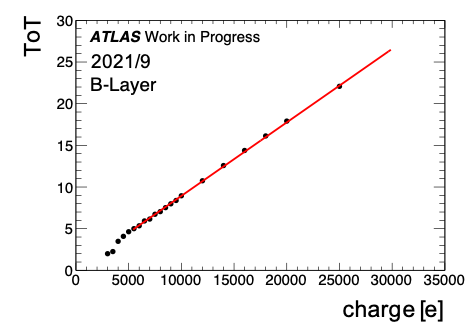
\includegraphics[keepaspectratio, scale=0.8]{blayernew1.png}
%  \end{minipage}
%  \begin{minipage}[b]{0.5\linewidth}
%    \centering
%    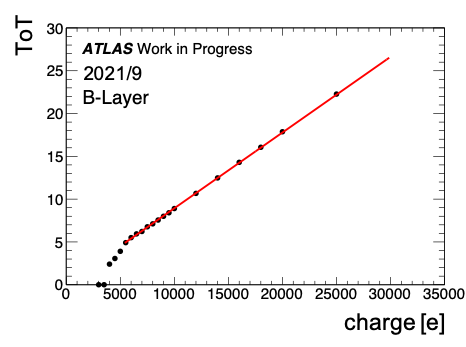
\includegraphics[keepaspectratio, scale=0.8]{blayernew2.png}
%  \end{minipage}
%  \caption[2021年9月に行われたB-Layerについての電荷較正結果]{2021年9月に行われたB-Layerについての電荷較正結果。}
%  \label{fig:blayernew}
%\end{figure}
%
%\fref{fig:blayernew}の左図は、Threshold値に近い小さい試験電荷量の点についてもToTから電荷量が再現できるものである。B-Layerではデジタル回路のThresholdとは別に、ToTの閾値が$3\ \si{ToT}$と定義されている。そのため、ToTが4以上であればデータの取得を行うが、そのようなものについても正しく較正できる。
%
%一方で、\fref{fig:blayernew}の右図は、Threshold値に近い小さい試験電荷量の点についてToTから電荷量の較正が正しくできないものである。ToTが5以上であれば、試験電荷から得られる点のフィット曲線上にあるため正しく較正できるが、$\mathrm{ToT}=4$の場合は、正しく較正できなくなってしまう。
%
%RUN2終了時までの電荷較正では電荷較正に用いられる試験電荷の最小値は$6000\ \si{e}$であり、電荷量を$2000\ \si{e}$ずつ変化させてデータの取得を行っていたため小さい試験電荷についての2つの構造が確認できていなかった。しかし、RUN3に向けた電荷較正では、放射線損傷による電荷収集の低下を保障するようThresholdを$3500\ \si{e}$まで引き下げられた。さらに、試験電荷の電荷量は$500\ \si{e}$ずつ変化させスキャンを行うため、このような違いが確認できるようになったと考えられる。そのため、小さい試験電荷を用いたToTスキャンについての理解を深め、\fref{fig:blayernew}の右図のような電荷較正結果が得られた際の電荷較正手法について再検討する必要があると考える。

%------------------------------------------------------------------------------------------------------------------------
\subsection{小さいToTに対する電荷較正}
\label{sec:minitot}
%------------------------------------------------------------------------------------------------------------------------

Run3に向けた電荷較正ではThreshold付近の電荷量を持つ試験電荷をより細かく生成した。電荷較正結果の再較正では$5000\ \si{e}$以下の試験電荷を全て取り除くことにより再較正が完了するため、$\mathrm{ToT}=5$以上の点は正しく電荷較正することが可能だが、それより小さいToTについては電荷較正のフィッティング結果と試験電荷の間に差異が現れた。この差異がデータ取得時の電荷較正にもたらす影響について本節で説明する。

ピクセル検出器におけるデータ取得では、タイムウォークの影響を抑えるためにIntime thresholdを用いており、1つのピクセルに対して電荷量がIntime threshold以下となる場合にはピクセルのヒット情報は記録されない。Run3に向けた電荷較正では、Intime threshldは約$4500\ \si{e}$となっており、Intime threshold以下の電荷量に相当するToTである$\mathrm{ToT}\leq3$についてはヒット情報は記録されない。よって、小さいToTにおける電荷較正の差異がデータに影響を与えるのは$\mathrm{ToT}=4$のみである。

$\mathrm{ToT}=4$における電荷較正を評価するために、\fref{fig:totsmall}に示すようにB-Layerの全FEチップについて電荷較正に用いたデータから$3.5 < \mathrm{ToT} < 4.5$となる点を取り出し、その電荷量と電荷較正\eref{eq:calibration}から得られる電荷量の比を計算した。その結果を\fref{fig:hikakukekkadayon}に示す。この図に示すように、データの電荷量と電荷較正\eref{eq:calibration}から得られる電荷量の比の分布には2つのピークが確認できた。これは、\fref{fig:blayernew}のように電荷較正結果のフィッティングには2つの構造があることだと考えられる。左の図の場合は、電荷較正結果が$\mathrm{ToT}=4$までデータ点を正しく再現できるものである。そのため、\fref{fig:hikakukekkadayon}において、データの電荷量と電荷較正\eref{eq:calibration}から得られる電荷量の比は$1$に近い値を持つ。一方で、\fref{fig:blayernew}の右図は、電荷較正結果が$\mathrm{ToT}=4$までデータ点を正しく再現できるものである。そのため、データの電荷量と電荷較正\eref{eq:calibration}から得られる電荷量の比は$1.2$に対応するものであり、この電荷較正結果がデータを再現するためにはフィッティング結果から得られる電荷量を$1.2$倍する必要がある。

\begin{figure}[tbp]
  \centering
  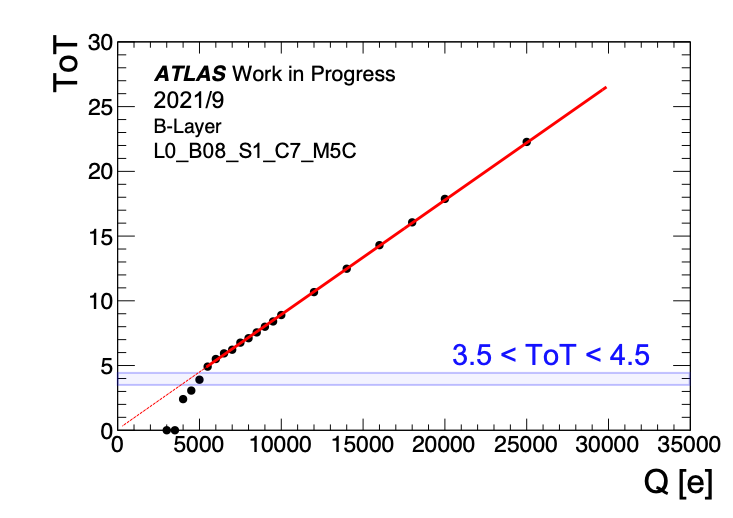
\includegraphics[height=7cm,keepaspectratio]{ToT34.png}
  \caption[$\mathrm{ToT}=4$における電荷較正の評価方法]{$\mathrm{ToT}=4$における電荷較正の評価方法。黒点は試験電荷のデータ点、赤線は$5500\ \si{e}$以上のデータ点を用いて作成したフィット結果を表す。青の領域は$3.5 < \mathrm{ToT} < 4.5$を表し、$\mathrm{ToT}=4$における電荷較正結果の評価のためにこの領域内の試験電荷のデータ点を取り出す。その試験電荷量とフィット結果から逆算される電荷量の比を計算することにより評価を行う。}
  \label{fig:totsmall}
\end{figure}

\begin{figure}[tbp]
  \centering
  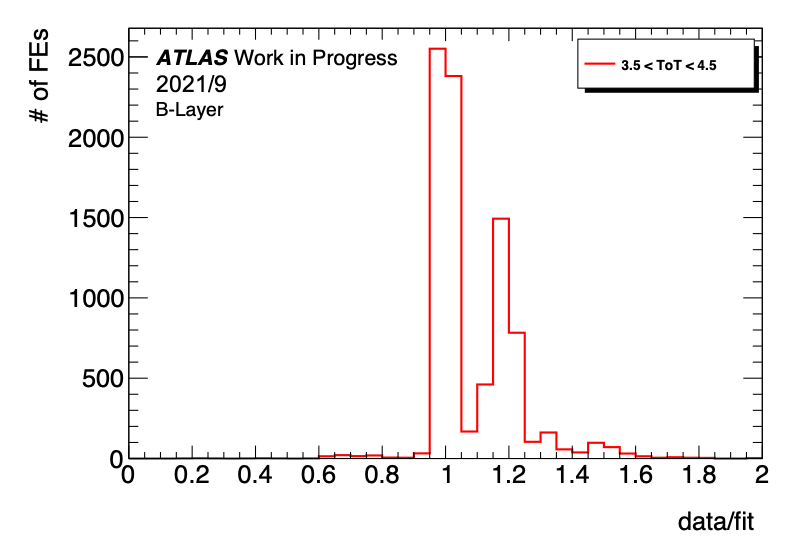
\includegraphics[height=7cm,keepaspectratio]{hikakukekkadayon.png}
  \caption[$\mathrm{ToT}=4$における電荷較正の評価結果]{$\mathrm{ToT}=4$における電荷較正の評価結果。横軸はデータの電荷量と電荷較正\eref{eq:calibration}から得られる電荷量の比を表し、縦軸はFEチップの数を表す。}
  \label{fig:hikakukekkadayon}
\end{figure}

\begin{figure}[tbp]
  \begin{minipage}[b]{0.5\linewidth}
    \centering
    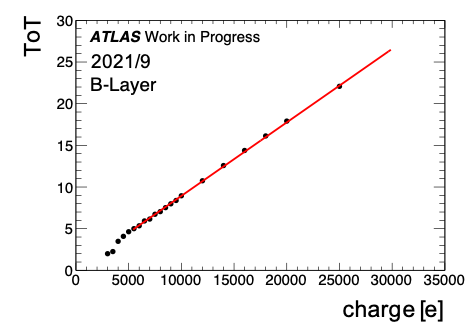
\includegraphics[keepaspectratio, scale=0.85]{blayernew1.png}
  \end{minipage}
  \begin{minipage}[b]{0.5\linewidth}
    \centering
    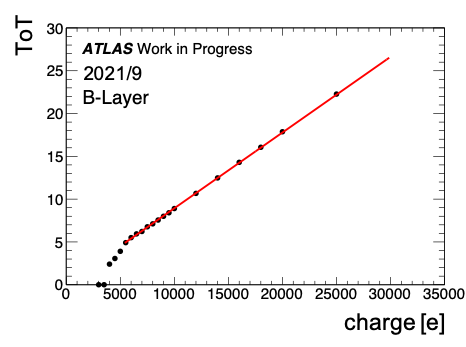
\includegraphics[keepaspectratio, scale=0.85]{blayernew2.png}
  \end{minipage}
  \caption[B-Layerの電荷較正結果における2つの異なる構造]{B-Layerの電荷較正結果における2つの異なる構造。左図は電荷較正結果が$\mathrm{ToT}=4$までデータ点を正しく再現できるものであり、右図は$\mathrm{ToT}=5$までデータ点を正しく再現できるものである。}
  \label{fig:blayernew}
\end{figure}

以上のことから、B-Layerについての電荷較正では、一部のFEチップについて$\mathrm{ToT}=4$の電荷較正結果を正確にデータ点を再現するためには、ToTから変換して得られる電荷量を約$1.2$倍する必要があることがわかった。しかし、以下の2つの理由から$\mathrm{ToT}=4$から得られる小さい電荷量の補正は行わないことに決定した。
\begin{itemize}
  \item MIP粒子に対する影響が大きくないと予想される\\
  荷電粒子が複数のピクセルにまたがりセンサーを通過すると、荷電粒子がセンサーに落とす電荷は複数のピクセルに分割される。そのため、荷電粒子の通過情報はヒットがあるピクセルのクラスターをつくることにより記録される。MIP粒子に相当する参照電荷量($20000\ \si{e}$)に対応するToTは$18$であるため、$\mathrm{ToT}=4$はクラスターの境界付近に現れる。$\mathrm{ToT}=4$に対する電荷量は約$20\%$ずれるため$1000\ \si{e}$程度の違いが現れるが、この電荷量はMIP粒子がシリコンセンサーに落とす電荷量のゆらぎ(\fref{fig:mipdist}参照)よりも十分小さい。そのため、$\mathrm{ToT}=4$から得られる小さい電荷の補正をしなくても、クラスターに対する影響は小さいと予想される。
  \item データベースを圧迫する\\
  全てのFEチップについて一律の倍率をかけることにより補正するのではなく、特定のFEチップにズレがあるため、そのFEチップのみに対して補正を行う必要がある。しかし、データベースにアップロードするパラメータの数は既に保存できる限界の量であり、これ以上増やすことができない。そのため、各FEチップに対して補正に必要な値を保存しておくことができず、小さい電荷を補正する値を保存しておくことができない。
\end{itemize}

\section{本章のまとめ}
本章では、電荷較正結果を確認し補完を行う解析ツールの概要を説明した。電荷較正の際に発生しうる問題は2種類ある。1つ目の問題は、電荷較正を行う際に正しい試験電荷が生成できないことである。この問題を検知するために電荷較正結果の新たな評価方法を導入し、問題のある試験電荷を順に取り除くアルゴリズムを開発した。2つ目の問題は、電荷較正結果に含まれるパラメータの欠損である。これまでの補完方法は最も近いFEチップから値をコピーするという方法であり、担当者により異なる値による補完を行ってしまうことがある。そのため、本研究においてパラメータの最適な補完方法の評価を行った。その結果、Threshold値については同一FEチップにおける異なるピクセルタイプの平均、その他のパラメータについては異なるFEチップにおける同一ピクセルタイプの平均を用いることにより、より実際の値に近い値を再現できるという結果が得られた。この結果を利用し、電荷較正結果に含まれるパラメータの欠損を自動補完する解析ツールの開発を行った。

2021年9月にRun3モンテカルロシミュレーションサンプル作成のための電荷較正データの取得がATLASにおいて行われた。このデータに対して本研究で開発した解析ツールを電荷構成データに使用し、電荷較正結果の作成した。この電荷較正結果を用いて、2021年末にRun3における検出器環境のモンテカルロシミュレーションサンプル作成が行われた。

Run3に向けた電荷較正ではThreshold付近の電荷量を持つ試験電荷をより細かく生成した。そのため、Run2終了時では確認できなかった小さい電荷量について、データの電荷量と電荷較正式によるフィット結果から得られる電荷量に差異が確認された。その差異がデータ取得時にどの程度影響を与えるかの評価を行った。その結果、MIP粒子に対する影響が大きくないと予想されること、およびFEチップごとに補正のためのパラメータの値が異なり、補正を行うようにパラメータを管理するとデータベースを圧迫してしまうことから、$\mathrm{ToT}=4$から得られる小さい電荷量について補正を行わないことに決定した。




\newpage
